% Afficher des recommendations concernant la syntaxe.
\RequirePackage[orthodox,l2tabu]{nag}
\RequirePackage{luatex85}
% Paramètres du document.
\documentclass[%
a5paper%                       Taille de page.
,11pt%                         Taille de police.
,DIV=15%                       Plus grand => des marges plus petites.
,titlepage=off%                 Faut-il une page de titre ?
%,headings=optiontoheadandtoc%  Effet des paramètres optionnels de section.
%,headings=small%
,parskip=false%
,openany%
]{scrbook}
\renewcommand*\partheademptypage{\thispagestyle{empty}}
\newcounter{facteur}\setcounter{facteur}{17}%%%%%%%%%%%%%% Paramètre pour la taille globale des partitions. par défaut : 17
%\usepackage{geometry}
\usepackage{gredoc,mudoc,lyluatex}
\usepackage{pdfpages,transparent,array,ltablex}
\usepackage{framed}
\usepackage{adaptateur}

%%%%%%%%%%%%%%%%%%%%%%% Paramètres variables %%%%%%%%%%%%%%%%%%%%%%%%%%%%%%%%%%%%%%%%%%%%%%%%%%
%%% Taille des partitions grégoriennes.                                                      %%
%\grechangedim{overhepisemalowshift}{.7mm}{scalable} %%Distance to place a a horizontal episema over a note in a low position in the space.Default: 0.02287 cm
%\grechangedim{hepisemamiddleshift}{1.4mm}{scalable} %%Distance to place a horizontal episema in the middle of a space. Default: 0.07206 cm
%\grechangedim{overhepisemahighshift}{2.1mm}{scalable} %% Distance to place a horizontal episema over a note in a high position in the space. Default: 0.10066 cm
%\grechangedim{vepisemahighshift}{2.1mm}{scalable} %% Distance to place a vertical episema in a high position in the space. Default: 0.06634 cm
%\grechangestafflinethickness{50} %%% epaisseur des lignes The default value is same as staff size.
\grechangestaffsize{\value{facteur}}%%%%% 
%%%%%%%%%%%%%%%%%%%%%%%%%%%%%%%%%%%%%%%%%%%%%%%%%%%%%%%%%%%%%%%%%%%%%%%%%%%%%%%%%%%%%%%%%%%%%%%
% Par souci de clarté, la définition des commandes est reportée dans un document annexe.

%\addtolength{\voffset}{2mm}\addtolength{\headsep}{-2mm}
%\setlength{\extrarowheight}{2mm}
\addto\captionsfrench{%
  \renewcommand{\indexname}{Index des chants}%
}

\pdfcompresslevel=9

\def\arraystretch{1.2}

%%%%%%% Commandes ajoutées assez explicites %%%%%%%%%%%%%%%%
\newcommand{\reponsegras}[2]{
    \versio{\textbf{#1}}{{#2}}
}
\newcommand{\imagecentre}[2]{
\begin{center} \includegraphics[height=#1]{img/#2} \end{center}}

%%%%%%%%%%% Pour la page de titre %%%%%%%%%%%%%
\title{\centrer{\huge{Veillée pascale}}}
\author{\includegraphics[height=10cm]{images/PâquesN-B.jpg}}
\date{la nuit de la Résurrection\\ avec baptêmes d'adultes}


\newcommand{\rep}[2]{\versio{\rb. \textbf{#1}}{\rb. \textbf{#2}}}
        \newcommand{\vers}[2]{\versio{\vb. {#1}}{\vb. {#2}}}
        
%%%insère une page blanche (saut d'une page entière ) 
\newcommand{\pageblanche}{
\newpage
\thispagestyle{empty}
\strut
\thispagestyle{empty}
\newpage
\thispagestyle{empty}}

\newcommand{\centrer}[1]{
    \vspace*{\stretch{1}}
#1
    \vspace*{\stretch{1}}}

%%%%%%%%%%%%%%%%%%%%%%%%%%%%%%%%%%%%%%%%%%%%%%%%%%%%%%%%%%%%%%%%%%%%%%%%%%%%%%%%
%%%%%%%%%%%%%%%%%%%%%%%%%%%%%%%%%%%%%%%%%%%%%%%%%%%%%%%%%%%%%%%%%%%%%%%%%%%%%%%%
%%%%%%%%%%%%%%%%%%%%%%%%%%%%%%%%%%%%%%%%%%%%%%%%%%%%%%%%%%%%%%%%%%%%%%%%%%%%%%%%
\begin{document}



\newfontfamily\malettrine[Scale=0.8]{l800}
\renewcommand{\LettrineFontHook}{\malettrine\color{black}}

\maketitle
\thispagestyle{empty}
\pageblanche

\titre{Bénédiction du feu et du cierge}
\vspace{0.5cm}
\rubrica{Le Christ, "lumière du monde" (Jn,8,12) va illuminer tout homme cette nuit en sortant du tombeau, il va dissiper les ténèbres du péché.}
\rubrica{Le prête bénit le feu, puis trace sur le cierge la croix, l'alpha et l'oméga, et les chiffres de l'année :}

\begin{center}
{
\scshape
\versio{Christus Heri et hodie}{Le Christ hier et aujourd'hui}
\versio{Princ\'ipium et Finis}{Commencement et Fin}
\versio{Alpha et Omega}{Alpha et Omega}
\versio{Ips\'ius sunt témpora et s\'æcula}{A lui sont les temps et les siècles}
\versio{Ipsi glória et impérium}{A Lui gloire et domination}
\versio{per univérsa æternit\'atis s\'æcula. Amen}{pendant tous les siècles de l'éternité. Amen}
}
\end{center}

\titre{Procession du cierge pascal}
\rubrica{Par trois fois le prêtre annonce la lumière qui jaillit, nous répondons pour manifester notre foi en Dieu, Père, Fils et Saint-Esprit :}
\versio{Lumen Christi !}{Lumière du Christ !}
\versio{\textbf{Deo Gratias !}}{\textbf{Nous rendons grâce à Dieu !}}

\rubrica{Alors la Lumière se répand par étape à travers toute l'église en allumant nos cierges au cierge bénit.}

\titre{Exsultet}
\nopagebreak
\rubrica{Alors le prêtre chante l'\emph{Exsultet}, chant de gloire et d'honneur à Jésus, Roi éternel, Lumière du monde, et Vainqueur des ténèbres.}
Qu'elle bondisse de joie, la multitude
des \emph{Anges} dans le ciel!
Qu'ils exultent, ces serviteurs de Dieu !
Et pour la victoire d'un si grand Roi,
que retentisse la trompette sacrée !

Que se réjouisse aussi \emph{la terre},
irradiée de si vives clartés : qu'illuminée par la splendeur du Roi éternel,
elle se sente dégagée des ténèbres
qui couvraient l'univers!

Que se réjouisse aussi notre mère
\emph{l'Eglise}, parée des rayons d'une telle
lumière! Et que cette enceinte résonne
sous les voix puissantes des fidèles!
\vspace{.5\baselineskip}

\cantus{Autre}{PerOmnia-ferial}{}{}

Il est vraiment juste et nécessaire
de faire servir nos voix à célébrer,
de toute l'affection du coeur et de
l'âme, le Dieu invisible, Père tout puissant,
et son Fils unique notre Seigneur Jésus-Christ, qui a payé d'Adam, et effacé de son sang précieux l'arrêt de l'antique péché.(...)

O admirable grandeur de votre tendresse envers nous! Ô faveur inestimable de votre
amour : pour délivrer l'esclave, vous livrez le Fils !
O péché d'Adam qui devait se commettre pour être effacé par la mort du Christ!
\emph{O heureuse faute qui nous a valu d'avoir un tel, un si grand Rédempteur !}


\titre{Les Lectures}

\rubrica{Nous nous rappelons différents passages de l'Ancien Testament figure du Nouveau.}
\begin{enumerate}
\item{La Création, symbole de notre régénération dans le Christ.}
\item{Le passage de la Mer Rouge, symbole de notre purification par le passage des eaux du Baptême dans lesquelles sont ensevelis tous nos péchés.}
\item{Les promesses rapportées par Isaïe, adressées au nouveau peuple élu.}
\item{Les recommandations que Moïse adresse à tous ceux qui feront ou renouvelleront les promesses de leur Baptême.}
\end{enumerate}


\titre{Litanies des Saints}
\rubrica{Avant la bénédiction de l'eau baptismale, et les baptêmes, invoquons tous nos aînés dans la Foi qui nous montrent l'exemple.}
\input{gabc/Litanies/litanies-1erePartie}

\titre{Bénédiction de l'eau baptismale}
\rubrica{Le prêtre chante une oraison puis une préface sur l'eau qui deviendra la matière du premier des sacrements, le Baptême.}
O Dieu, dont l'Esprit, à l'origine du
monde, planait sur les eaux, pour
leur donner déjà le pouvoir de nous
sanctifier. Ô Dieu, qui en lavant
par l'eau les crimes d'un monde coupable, avez donné, dans l'inondation
même du déluge, une image de la
régénération, alors que dans le mystère d'un seul et même élément se voyaient tout ensemble et la. ruine
du vice et le principe de la vertu.
Regardez, Seigneur, la face de votre
Eglise et multipliez en elle vos régénération.


\rubrica{Le célébrant, de la main étendue, divise l'eau en forme de croix. Ainsi
Dieu en créant le monde avait séparé les eaux d'en-haut de celles d'en bas.}
Qu'il vienne, par la secrète union de sa divinité, féconder cette eau préparée pour la régénération des hommes.


\rubrica{Il touche l'eau avec la main. Le Christ, en touchant l'eau du Jourdain, lui a enlevé toute puissance nocive; elle est devenue le signe et l'instrument de notre délivrance.}
Que cette eau soit
une source de vie, une eau qui
régénère, une onde purifiante, afin
que tous ceux qui seront lavés dans
ce bain salutaire, reçoivent, par l'opération du Saint-Esprit qui agira en
eux, la grâce d'une entière purification.

\rubrica{Il fait trois signes de croix sur l'eau, en disant:}
\versio{Unde benedíco te, creatúra aquæ, per Deum \x~vivum, per Deum \x~verum, per Deum \x~sanctum : per Deum, qui te in princípio verbo separávit ab árida : cuius Spíritus super te ferebátur.}
{Je te bénis donc, eau créée, par
le Dieu \x~vivant, par le Dieu
vrai, par le Dieu \x~saint : par \x~le Dieu, dont la parole te sépara de
la terre à l'origine et dont l'Esprit planait sur toi.}

\rubrica{Ici, il divise l'eau avec la main et en jette vers les quatre parties du monde,
Ce geste rappelle le fleuve qui, sorti de l' Eden, se divisait en quatre branches,
pour arroser « la terre entière ».}

\rubrica{Il plonge ensuite trois fois le cierge dans l'eau, pour rappeler que le Christ
a sanctifié les eaux en descendant dans le Jourdain et que la Sainte Trinité
s'est manifestée à ce moment; il chante à chaque fois : }
\versio{Descéndat in hanc plenitudinem fontis virtus Spiritus Sancti}{
Que la vertu du Saint-Esprit descende sur toute l'eau de cette fontaine.}

\rubrica{Puis le prêtre extrait de l'eau qui servira tout le temps pascal, et termine la consécration de l'eau par l'infusion des Huiles consacrées le Jeudi Saint par l'évêque.}

\versio{Sanctificétur et fecundétur
fons iste Oleo sal\'utis renascéntibus ex eo, in vitam ætérnam.}
{Que cette fontaine soit sanctifiée et fécondée par l'Huile du salut pour ceux qui y renaîtront à la vie éternelle.}
\reponsegras{\rb. Amen.}{\rb. Ainsi soit-il.}

\versio{
Infusio Chrismatis D\'omini 
nostri Jesu Christi, et Spiritus 
Sancti Paracliti, fiat in n\'omine 
sanctæ Trinit\'atis.}
{Que l'infusion du Chrême de notre Seigneur Jésus-Christ et de l'Esprit-Saint Consolateur, se fasse au nom de la sainte Trinité.}
\reponsegras{\rb. Amen.}{\rb. Ainsi soit-il.}

\versio{
Commixtio Chrismatis sanctificati\'onis, et Olei uncti\'nis, et aquæ bapt\'ismatis, p\'ariter fiat in n\'omine Pa\x tris, et
Fi\x lii, et Spiritus \x~ Sancti.}{
Que le mélange du Chrême sanctifiant, de l'Huile d'onction et
de l'eau baptismale s'opère également
au nom du Père, \x~ et du Fils, \x~ et
du Saint \x~ Esprit. }
\reponsegras{\rb. Amen.}{\rb. Ainsi soit-il.}

\titre{Le Sacrement de Baptême}
\rubrica{Le prêtre administre alors le sacrement de Baptême aux catéchumènes.}
\textsc{Le célébrant :} - Croyez-vous en Dieu, le Père tout-puissant,
Créateur du ciel et de la terre?

\textsc{Le catéchumène :} - J'y crois.

- Croyez-vous en Jésus-Christ, son Fils unique, notre
Seigneur, qui est né et quui est mort pour nous

- J'y crois.

- Croyez-vous au Saint-Esprit, à la Sainte Église
catholique, à la communion des Saints, à la rémission
des péchés, à la résurrection de la chair et à la vie
éternelle?

- J'y crois.

- Voulez-vous être baptisé ?

- Je le veux.

\rubrica{Le célébrant verse de l'eau baptismale par trois fois sur la tête de celui qui
doit êre baptisé, en disant en latin :}
%\textsc{\rubrum{N.},\nigra{} JE VOUS BAPTISE AU NOM DU PÈRE, ET DU FILS, ET DU SAINT ESPRIT.}

%\scalebox{.91}[1]{\textsc{\addfontfeatures{Renderer=Basic}\rubrum{N.},\nigra{} JE VOUS BAPTISE AU NOM DU PÈRE, ET DU FILS, ET DU SAINT ESPRIT.}}\par%

\versio{%
{\red N.}{}, EGO TE BAPTISO IN NOMINE PATRIS ET FILII ET SPIRITUS SANCI.}%
{%
{\red N.}, JE VOUS BAPTISE AU NOM DU PÈRE, ET DU FILS, ET DU SAINT ESPRIT.}%


\titre{Renouvellement des promesses du baptême}
\rubrica{Alors, tous nous sommes invités à renouveler la promesse de fidélité à Dieu.}

\newpage
\titre{Deuxième partie des litanies}
\rubrica{On termine alors les litanies, en demandant la protection divine ; pendant ce temps, le chœur est préparé pour la messe de la Résurrection.}

\input{gabc/Litanies/litanies-2emePartie}

\cleardoublepage
\titre{Messe de la Résurrection}
\begin{center}
\includegraphics[height=7cm]{images/Pâques2N-B}
\end{center}
\rubrica{Après nous avoir fait revivre la grâce de notre baptême, l'Eglise nous invite à offrir avec elle le saint sacrifice de la messe. C'est l'action de grâces, où nous présentons à Dieu l'Agneau pascal, immolé pour le salut du monde.}

\subsection*{Kyrie}
\cantus{Kyriale}{Kyrie-I}{I}{}
\subsection*{Gloria}
\rubrica{C'est au moment du Gloria que la joie pascale est complète, les cloches sonnent à nouveau, l'orgue se réveille, et toutes les statues quittent leur voile de deui.l}

Gloire à Dieu au plus haut des cieux, et paix sur la terre aux hommes de bonne volonté. 
Nous vous louons, nous vous bénissons, nous vous adorons, nous vous glorifions. 
Nous vous rendons grâces pour votre gloire immense, Seigneur Dieu, Roi du ciel, Dieu Père tout-puissant. 
Seigneur Fils unique, Jésus-Christ, Seigneur Dieu, Agneau de Dieu, Fils du Père, vous qui enlevez les péchés du monde, ayez pitié de nous ; vous qui enlevez les péchés du monde, accueillez notre prière ; vous qui siégez à la droite du Père, ayez pitié de nous. 
Car vous êtes le seul Saint, le seul Seigneur, le seul Très-Haut, Jésus-Christ, avec le Saint-Esprit, dans la gloire de Dieu le Père. Ainsi soit-il.
\cantus{Kyriale}{Gloria-I}{I}{}

\subsection*{Oraison}
Ô Dieu, qui illuminez cette très sainte nuit de la gloire de la résurrection du Seigneur, conservez dans les nouveaux enfants de votre famille l’esprit d’adoption que vous leur avez donné ; afin que, renouvelés de corps et d’esprit, ils vous servent dans l’innocence. Par le même Jésus-Christ Notre-Seigneur.

\subsection*{Epître}
\rubrica{Saint Paul nous invite à vivre et à renouveller la grâce de Dieu en nous : vivons en ressuscités.}

\subsection*{Alleluia}
\rubrica{Unissons-nous avec le prêtre, en reprenant l'Alleluia}
\cantus{Alleluia}{Confitemini_Quoniam_SabbatoSancto_jubilus}{VIII}{}
Célébrez le Seigneur, parce qu’il est bon, parce que sa miséricorde est éternelle.

Nations, louez toutes le Seigneur ; peuples, louez-le tous. Car sa miséricorde a été affermie sur nous, et la vérité du Seigneur demeure éternellement.

\subsection*{Evangile}
\nopagebreak
\rubrica{Récit de la découverte de la Résurrection}

\subsection*{Offertoire}
\rubrica{À l'Offertoire l'Église offre le Corps et le Sang du Christ, représentés par le pain et le vin. Notre Seigneur a communiqué à son Église le pouvoir d'offrir le même sacrifice qu'il offrit sur la Croix. L'Église s'y unit comme victime. \emph{Le Christ lui-même est à la fois le prêtre qui offre et la victime qui est offerte. Le sacrifice de l'Église est le sacrement quotidien du sacrifice du Christ. L'Église, qui est le corps dont il est la tête, s'y offre elle-même par lui. C'est pourquoi dans ce sacrement l'Église elle-même est offerte dans ce qu'elle offre.} (S.~Augustin). Nous sommes donc une seule victime avec le Christ, unissant nos propres offrandes et nos sacrifices à celui du Christ et de l'Église.}
Recevez, Père saint, Dieu éternel et tout-puissant, cette offrande sans tache, que moi, votre indigne serviteur, je vous présente, à vous, mon Dieu vivant et vrai, pour mes péchés, offenses et négligences sans nombre, pour tous ceux qui m'entourent, ainsi que pour tous les fidèles vivants et morts : qu'elle serve à mon salut et au leur pour la vie éternelle. Ainsi soit-il.

\rubrica{Le prêtre prépare le calice en y versant le vin ; il y ajoute quelques gouttes d'eau qu'il bénit. L'eau mêlée au vin figure l'union en Jésus-Christ de la nature humaine à la personne divine, et symbolise aussi le chrétien intimement uni au Christ. Le vin et l'eau rappellent le Sang et l'eau qui coulèrent du côté du Christ percé par la lance. \emph{Quand le vin et l'eau sont mêlés dans le calice, le peuple est uni au Christ et la foule des croyants est associée et réunie à celui en qui elle croit.} (S.~Cyprien)}
Dieu, ✠ qui, d'une manière admirable, avez créé la nature humaine dans sa noblesse, et l'avez restaurée d'une manière plus admirable encore, accordez-nous, selon le mystère de cette eau et de ce vin, de prendre part à la divinité de celui qui a daigné partager notre humanité, Jésus-Christ votre Fils, Notre Seigneur, qui, étant Dieu, vit et règne avec vous en l'unité du Saint-Esprit, dans tous les siècles des siècles. \mbox{Ainsi soit-il}.\looseness=1

\subsection*{Encensement}

\rubrica{Comme l'encens, consumé par le feu, s'élève en vapeur odorante, ainsi l'Église avec le Christ, consumée par le feu du Saint-Esprit, s'élève en sacrifice envers Dieu. On encense les oblats (le pain et le vin), puis l'autel, le prêtre, et enfin le clergé et les fidèles.}

\subsection*{%
Oraison silencieuse (Secrète)%
}
Agréez, nous vous en supplions. Seigneur, les prières de votre peuple avec l’oblation de ces hosties, en sorte qu’empreintes de l’esprit du mystère pascal, elles nous servent, grâce à votre action, de remède pour l’éternité.


\subsection*{%
Préface%
}
\rubrica{Par le chant de la Préface le prêtre rend grâces à Dieu au nom de l'Église pour l'œuvre du salut réalisée par Jésus-Christ.}

\versio{%
℣. Per ómnia sǽcula sæculórum. ℟. Amen.}{%
℣. Dans tous les siècles des siècles. ℟. Ainsi soit-il.}

\versio{%
℣. Dóminus vobíscum.}{%
℣. Le Seigneur soit avec vous.}

\versio{%
℟. Et cum spíritu tuo.}{%
℟. Et avec votre esprit.}

\versio{%
℣. Sursum corda.}{%
℣. Élevons nos cœurs.}

\versio{%
℟. Habémus ad Dóminum.}{%
℟. Ils sont tournés vers le Seigneur.\looseness=-1}

\versio{%
℣. Grátias agámus Dómino Deo nostro.}{%
℣. Rendons grâces au Seigneur notre Dieu.}

\versio{%
℟. Dignum et iustum est.}{%
℟. C'est juste et nécessaire.}

Il est vraiment juste et nécessaire,
c’est notre devoir et c’est notre salut,
de vous louer, Seigneur, en tout temps,
mais surtout avec encore plus de gloire en cette nuit
où le Christ, notre Pâque, a été immolé.
Car il est le véritable Agneau
qui a ôté les péchés du monde.
Il a détruit notre mort par la sienne
et nous a rendu la vie en ressuscitant.
C’est pourquoi, avec les Anges et les Archanges,
avec les Trônes et les Dominations,
et avec toute la milice de l’armée céleste
nous chantons l’hymne de votre gloire
en disant sans cesse :

\subsection*{Sanctus}
\vulgo{Saint, saint, saint le Seigneur, Dieu des armées. Les cieux et la terre sont remplis de votre gloire ; hosanna au plus haut des cieux ! Béni soit celui qui vient au nom du Seigneur ; hosanna au plus haut des cieux !}
\cantus{Kyriale}{Sanctus-I}{IV}{}

\subsection*{Canon}
\rubrica{Canon signifie règle. Cette partie de la messe est une règle intangible. Les prières du Canon remontent au-delà du VI\ieme{} siècle, voire pour certaines à l'Apôtre Pierre lui-même.}

\rubrica{À cet instant commence le rite consécratoire proprement dit. Il convient de se tenir à genoux. Le prêtre étend les mains sur le pain et le vin, comme faisait le Grand Prêtre de l'Ancien Testament sur la victime que l'on immolait pour l'expiation des péchés. Jésus-Christ a pris sur lui nos péchés pour les expier.}

Ainsi donc, Seigneur, ce sacrifice que nous vous offrons et, avec tous vos enfants, aujourd’hui spécialement pour ceux que vous avez daigné régénérer par l’eau et l’Esprit-Saint en leur accordant la rémission de tous leurs péchés, acceptez-le avec bienveillance ; disposez dans votre paix les jours de notre vie ; veuillez nous arracher à l'éternelle damnation et nous compter au nombre de vos élus. Par le Christ notre Seigneur. Ainsi \mbox{soit-il}.

\rubrica{Le prêtre récite alors l'histoire de l'institution de l'eucharistie en accomplissant les mêmes gestes que le Christ.}

\versio{%
Qui prídie quam paterétur, accépit panem in sanctas ac venerábiles manus suas, et elevátis óculis in cælum ad te Deum Patrem suum omnipoténtem, tibi grátias agens, bene ✠ díxit, fregit, dedítque discípulis suis, dicens : Accípite, et manducáte ex hoc omnes.}{%
Celui-ci, la veille de sa Passion, prit du pain dans ses mains saintes et adorables, et, les yeux levés au ciel vers vous, Dieu, son Père tout-puissant, vous rendant grâces, il ✠ bénit ce pain, le rompit et le donna à ses disciples en disant : Prenez et mangez-en tous.}


\rubrica{Le prêtre prononce alors les paroles mêmes de Notre-Seigneur. Par ces paroles il opère la conversion du pain au saint Corps du Christ.}

\versio{%
\scalebox{.91}[1]{\textsc{\addfontfeatures{Renderer=Basic}Hoc est enim Corpus meum.}}\par%
}{%
\textsc{\addfontfeatures{Renderer=Basic}Car ceci est mon Corps.}\par%
}

%\vspace{1\baselineskip plus 2\baselineskip}

\rubrica{Ces paroles étant prononcées, le prêtre fait la génuflexion pour adorer le saint Corps, l'élève pour le présenter à l'adoration des fidèles, le dépose sur l'autel et fait de nouveau la génuflexion. Le prêtre reprend le récit de l'institution de l'eucharistie :}

\versio{%
Símili modo postquam cenátum est, accípiens et hunc præclárum Cálicem in sanctas ac venerábiles manus suas : item tibi grátias agens, bene ✠ díxit, dedítque discípulis suis, dicens : Accípite, et bíbite ex eo omnes.}{%
De même, après le repas, il prit aussi ce précieux calice dans ses mains saintes et adorables, vous rendit grâces encore, le ✠ bénit et le donna à ses disciples en disant : Prenez et buvez-en tous.}

\rubrica{Prononçant alors les paroles mêmes de Notre-Seigneur, le prêtre opère la conversion du vin au précieux Sang du Christ.}
%
\nopagebreak\smallskip%
%
\versio{%
\textsc{\addfontfeatures{Renderer=Basic}Hic est enim Calix Sánguinis mei, novi et ætérni Testaménti : mystérium fídei : qui pro vobis et pro multis effundétur in remissiónem peccatórum.}%
}{%
\textsc{\addfontfeatures{Renderer=Basic}Car ceci est le Calice de mon Sang, le Sang de l'Alliance nouvelle et éternelle, le mystère de la foi, qui sera versé pour vous et pour un grand nombre en rémission des péchés.}%
}

\smallskip

\versio{%
Hæc quotiescúmque fecéritis, in mei memóriam faciétis.}{%
Toutes les fois que vous ferez cela, vous le ferez en mémoire de moi.}%

%\vspace{1\baselineskip plus 2\baselineskip}

\rubrica{Ces paroles étant prononcées, le prêtre fait la génuflexion pour adorer le précieux Sang. Il l'élève pour le présenter à l'adoration, et fait de nouveau la génuflexion.\\
\emph{Avant la consécration, ceci est du pain~; dès que sont intervenues les paroles du Christ, c'est le Corps du Christ. Avant les paroles du Christ, le calice contient du vin et de l'eau ; dès que les paroles du Christ ont agi, il contient le Sang qui a racheté le peuple.} (S. Ambroise)}

Nous vous en supplions, Dieu tout-puissant, faites porter ces offrandes par les mains de votre saint ange, là-haut, sur votre autel, en présence de votre divine Majesté. Et quand nous recevrons, en communiant ici à l'autel, le Corps ✠ et le Sang ✠ infiniment saints de votre Fils, puissions-nous tous être comblés des grâces et des bénédictions du ciel. Par le Christ notre Seigneur. Ainsi soit-il.

\subsection*{Memento des morts}
Souvenez-vous aussi, Seigneur, de vos serviteurs et de vos servantes N. et N., qui sont partis avant nous, marqués du sceau de la foi, et qui dorment du sommeil de la paix. À ceux-là, Seigneur, ainsi qu'à tous ceux qui reposent dans le Christ, accordez, nous vous en supplions, le séjour du bonheur, de la lumière et de la paix. Par le Christ notre Seigneur. Ainsi soit-il.

\rubrica{C'est par ce Sacrifice que toute gloire est rendue à Dieu par le Christ. Le prêtre élève l'hostie et le calice, après avoir tracé avec l'hostie trois signes de croix sur le calice, puis deux signes de croix devant le calice.}

\versio{%
Per ip ✠ sum, et cum ip ✠ so, et in ip ✠ so, est tibi Deo Patri ✠ omnipoténti, in unitáte Spíritus ✠ Sancti, omnis honor, et glória.}{%
Par ✠ lui, avec ✠ lui, et en ✠ lui, vous sont donnés, Dieu Père ✠ tout-puissant, dans l'unité du ✠ Saint-Esprit, tout honneur et toute gloire.}

%\needspace{2\baselineskip}\pagebreak[1]
\rubrica{En répondant \emph{Amen} à cette conclusion du Canon, nous adhérons à l'œuvre sacrée qui vient de s'accomplir.}

\versio{%
℣. Per ómnia sǽcula sæculórum.}{%
℣. Dans tous les siècles des siècles.}

\versio{%
℟. Amen.}{%
℟. Ainsi soit-il.}


\needspace{9\baselineskip}
\subsection*{Pater  Noster}
\rubrica{\emph{Ô très grand amour de Dieu pour les hommes ! À ceux qui l'avaient abandonné il a accordé un tel pardon, une telle part de grâces, qu'il se fait appeler Père.} (S. Cyrille de Jérusalem). Au nom de l'Église le prêtre chante la prière que Jésus-Christ nous a apprise.}
\rubrica{\textbf{Dans les rites latins le Notre Père a toujours été chanté par le prêtre seul.}}

\versio{%
Orémus. Præcéptis salutáribus móniti, et divína institutióne formáti, audémus dícere :}{%
Prions. Éclairés par le commandement du Sauveur et formés par l'enseignement d'un Dieu, nous osons dire :}

\versio{%
Pater noster, qui es in cælis : sanctificétur nomen tuum ; advéniat regnum tuum~; fiat volúntas tua sicut in cælo et in terra.
Panem nostrum quotidiánum da nobis hódie ; et dimítte nobis débita nostra, sicut et nos dimíttimus debitóribus nostris. Et ne nos indúcas in tentatiónem.}{%
Notre Père, qui êtes aux cieux, que votre nom soit sanctifié, que votre règne arrive, que votre volonté soit faite sur la terre comme au ciel. Donnez-nous aujourd'hui notre pain de chaque jour ; pardonnez-nous nos of\-fen\-ses comme nous par\-don\-nons à ceux qui nous ont offensés ; et ne nous laissez pas succomber à la tentation.%
}
\reponsegras{%
\rb. Sed líbera nos a malo.}{%
\rb. Mais délivrez-nous du mal.}

\subsection*{Communion}
\rubrica{Après avoir communié, le prêtre se retourne vers les fidèles en leur présentant le saint Corps du Christ. \emph{En offrant Jésus-Christ à nos yeux, le prêtre nous révèle comment le Christ lui-même est sorti de son mystérieux sanctuaire divin pour prendre par amour de l'homme la nature de l'homme, pour s'incarner totalement sans se mélanger d'aucune façon.} (Denys l'Aréopagite)}

\versio{%
Ecce Agnus Dei, ecce qui tollis peccáta mundi.}{%
Voici l'Agneau de Dieu, voici celui qui enlève les péchés du monde.}

\rubrica{Nous répondons par les paroles du bienheureux centurion. Cette fois ce n'est plus la guérison d'un serviteur que nous demandons, mais celle de notre âme.}
%
\reponsegras{%
Dómine, non sum dignus, ut intres sub tectum meum : sed tantum dic verbo, et sanábitur ánima mea. \emph{ter}}{%
Seigneur, je ne suis pas digne que vous entriez sous mon toit ; mais dites seulement une parole, et mon âme sera guérie. \emph{ter}}

\rubrica{Aux premiers siècles le diacre invitait ceux qui ne communiaient pas à se retirer : \emph{les choses saintes aux saints, hors d'ici les impurs}, ou encore : \emph{que celui qui ne communie pas se retire}. Aujourd'hui l'Église est plus indulgente mais les conditions pour communier sont les mêmes : \textbf{être baptisé et catholique~; ne pas avoir de péché mortel sur la conscience, ce qui suppose notamment l'observation des lois de l'Église au sujet du mariage~; avoir observé le jeûne eucharistique.} La discipline actuelle est d'une heure de jeûne avant la communion. Nous conseillons cependant de s'en tenir à la discipline d'avant le Concile Vatican II : trois heures pour la nourriture solide, une heure pour le liquide non alcoolisé. La discipline antique (en vigueur jusqu'au milieu du XX\ieme{} siècle) exigeait d'être à jeun depuis minuit.\\
La sainte communion est reçue à genoux et directement dans la bouche.}

\subsection*{Action de grâces - Laudes}

\cantus{Antienne}{AlleluiaAlleluiaAlleluia}{VI}{}
\ps{150}
\vulgo{Louez le Seigneur dans son sanctuaire ; louez-le sur le trône inébranlable de sa puissance.}
\cantus{Psaume}{Intonation-150-6F}{6 F}{}
\psalmusversio[tonus=6F,monprimus=2,monnumerus=2]{150-t}
\mongloria[tonus=6F]

%\begin{center}
%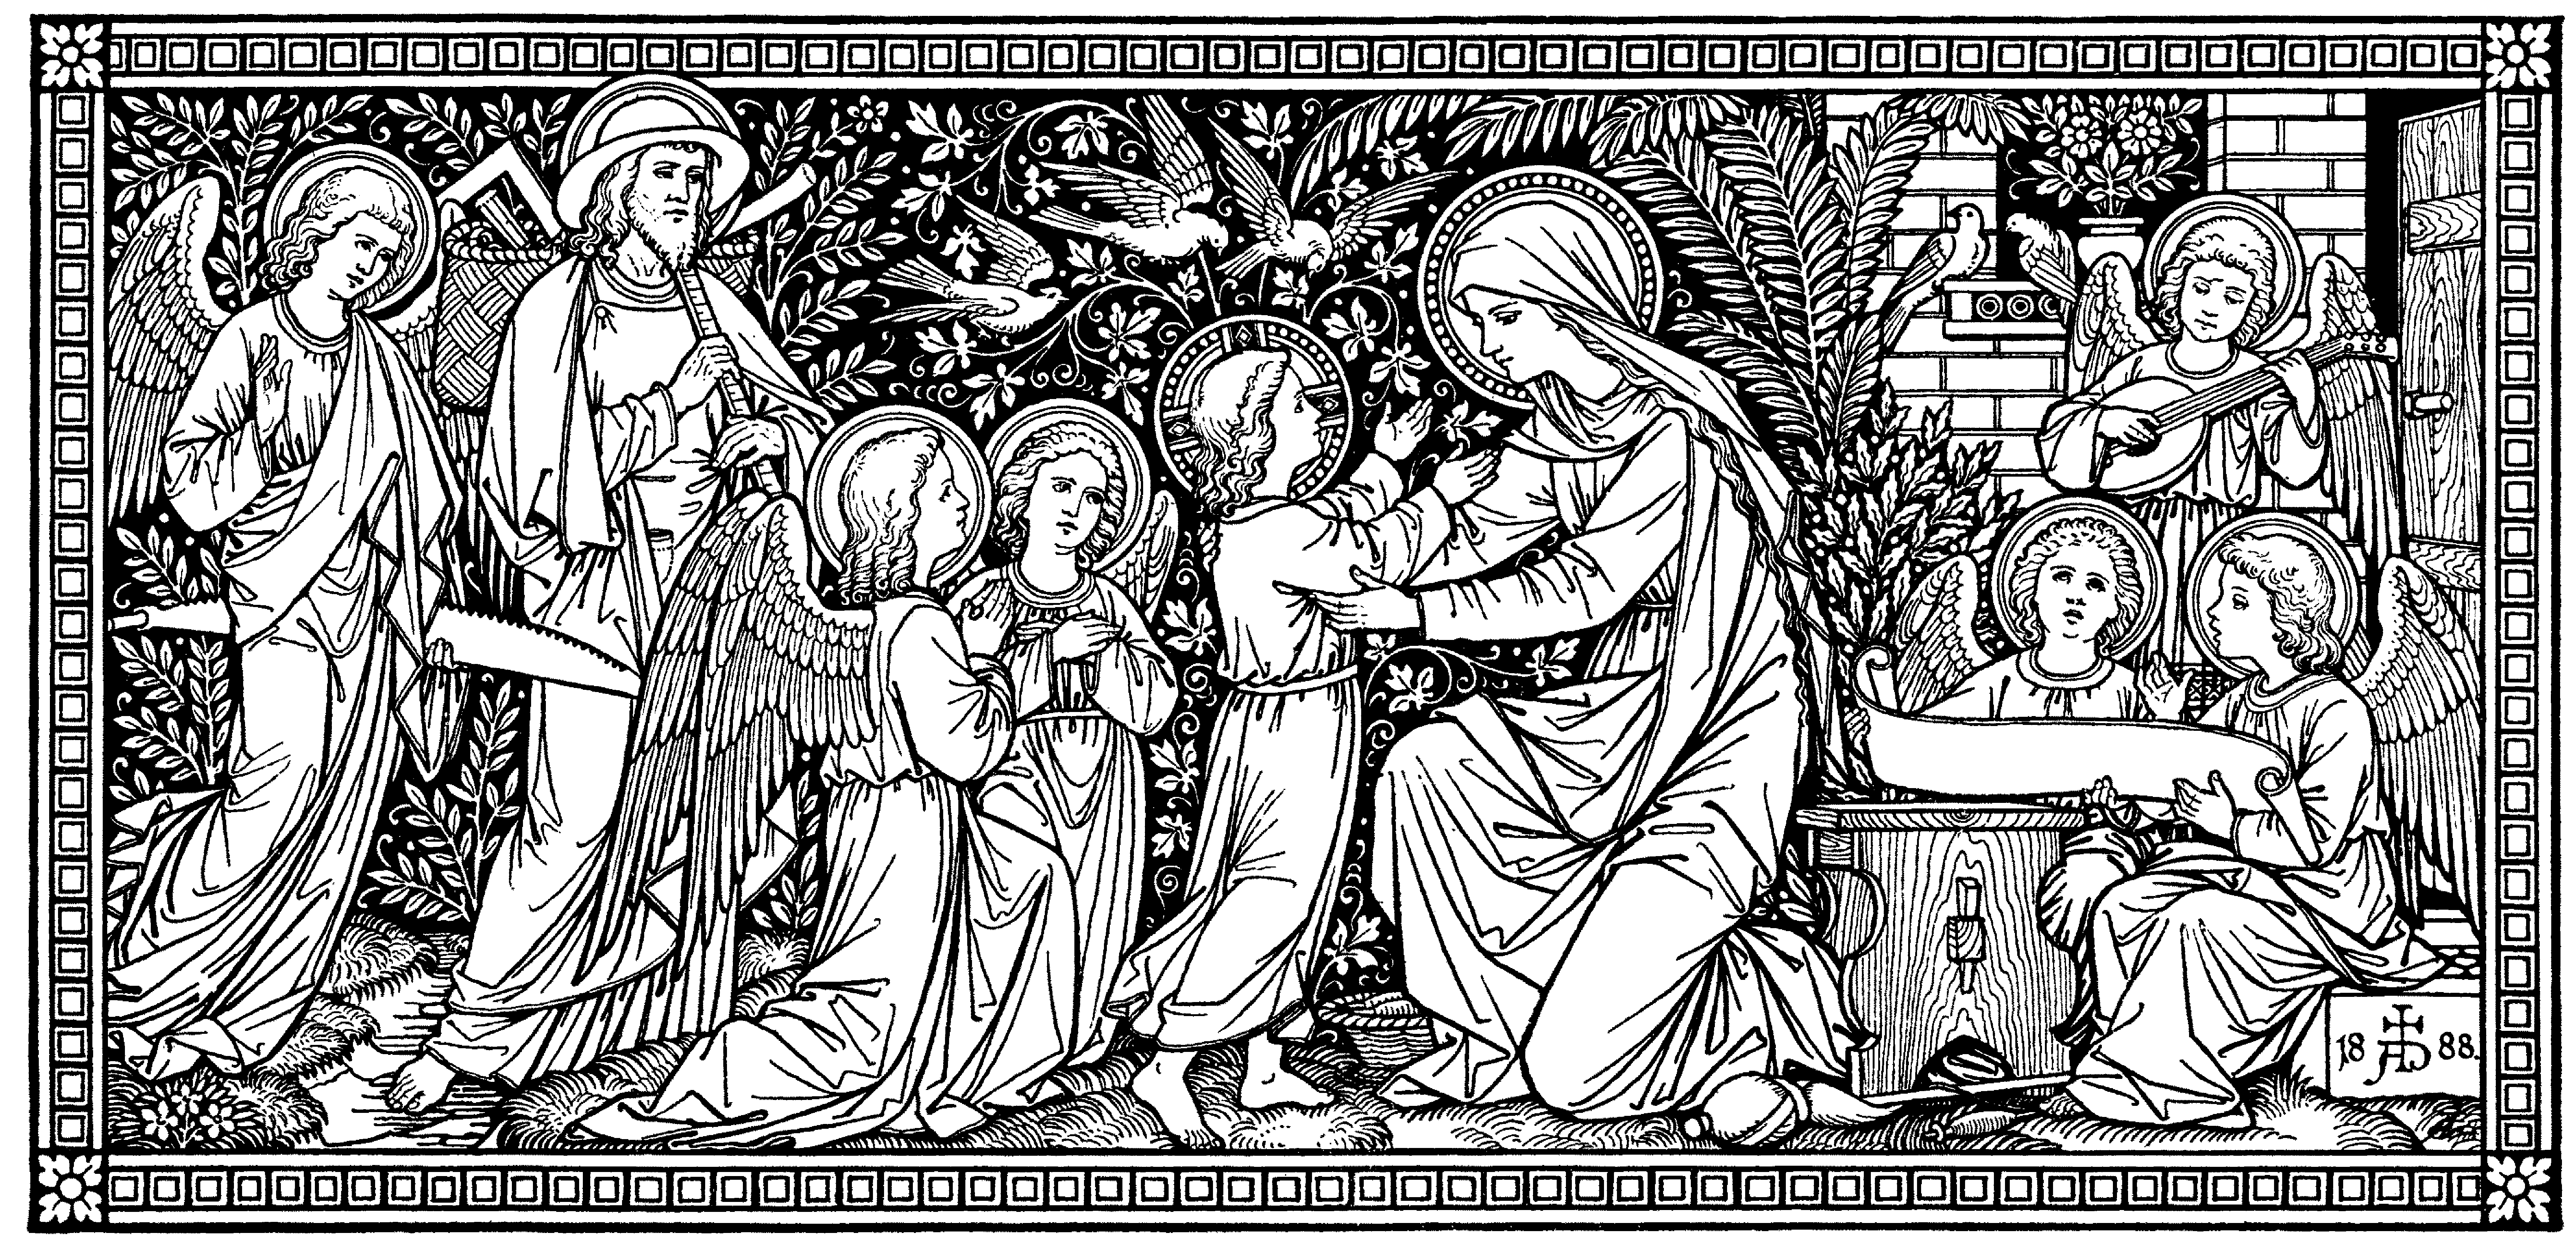
\includegraphics[height=5.5cm]{images/SainteFamille}
%\end{center}
\newpage
\thispagestyle{empty}
\begin{center}
\centrer{
\includegraphics{images/AgneauN-B}}
\end{center}

\end{document}
